\documentclass[12pt]{paper}
\RequirePackage{filecontents}
\begin{filecontents}{pp.bib}
	@misc{
		PWA,
		author = {{Sam Richard, Pete LePage}},
		year = {2020},
		title = {{Progressive Web App}},
		note= {\url{https://web.dev/what-are-pwas/}}
	}
	@protocol{
		openid,
		title = {{OpenId Connect}},
		year = {2007},
		author = {{Brad Fitzpatrick}},
		note = {\url{https://openid.net/}}
	}
\end{filecontents}
\usepackage{graphicx}
\usepackage{hyperref}
\usepackage[english]{babel}
\usepackage{setspace}
\usepackage{indentfirst}
\usepackage[utf8]{inputenc}
\usepackage{fancyhdr}
\usepackage{tabu}
\usepackage{setspace}
\pagestyle{plain}
\fancyhf{} % sets both header and footer to nothing
\renewcommand{\headrulewidth}{0pt}
\usepackage[document]{ragged2e}
\pagenumbering{arabic}
\usepackage[hmargin=2.5cm,vmargin=2.5cm,bmargin=2.5cm]{geometry}
\title{
	\vspace{-50mm}
	\begin{minipage}[l]{\textwidth}
		\hspace{-20mm}\resizebox{75mm}{!}{
\includegraphics{./images/logoISEL.png}}
	\end{minipage}
}

\author{
	\begin{tabular}{ll}
		& Bernardo Rodrigues\\[50mm]
	\end{tabular}
}

\date{
	\begin{tabular}{ll}
		{Supervisors: }&& Nuno Leite\\
	\end{tabular}[10mm]
}



\begin{document}
	\begin{titlepage}
		\begin{figure}[!ht]
			\centering
			\hspace{-20mm}\resizebox{75mm}{!}{
\includegraphics{./images/logoISEL.png}}\\
%			\scalebox{0.6}{\includegraphics{images/Logo_ISEL}}
		\end{figure}	
		
		\begin{center}
			%TODO maybe change name
			{\huge TODO}\\
			\vspace{1.5cm}
			{\Large Engenharia Informática e Computadores}\\
			{\large Projecto e Seminário - 2020/21}
		\end{center}
	
		\vspace{1cm}
	
		\begin{center}
			
		\end{center}
		
		\vspace {0.1cm}
		\begin{itemize}
			\item[] Bernardo Rodrigues, n. 42130
			\\ \href{mailto:bernardo.qtr.21@gmail.com}{bernardo.qtr.21@gmail.com}
		\end{itemize}
		\vspace{1cm}
		\begin{center}
			\centering
			Supervisors:
			\\
			Nuno Leite, ISEL, \href{mailto:nuno.leite@isel.pt}{nuno.leite@isel.pt}
		\end{center}
		
		\rfoot{\today}
	\end{titlepage}

	\section{State of the Art}

	\setcounter{page}{2}
	\section{Introduction}
	Today's world is a fast, complex moving mess. As such we try to schedule our days or weeks, or we create small reminders to do something, whatever that may be. Those little notes we give ourselves, those "to-do's" are often forgotten and not fully fulfilled. As such this application will attempt to mend that by creating an environment where a reminder is easily created but hardly forgotten or skipped over.
		
	\section{Proposed Solution}
		The goal of the project is to create a web application using current practices and technologies. The application will be comprised of a web \textit{API}, a database and front-end application as shown below.
		\begin{figure}[!h]
			\centering
			%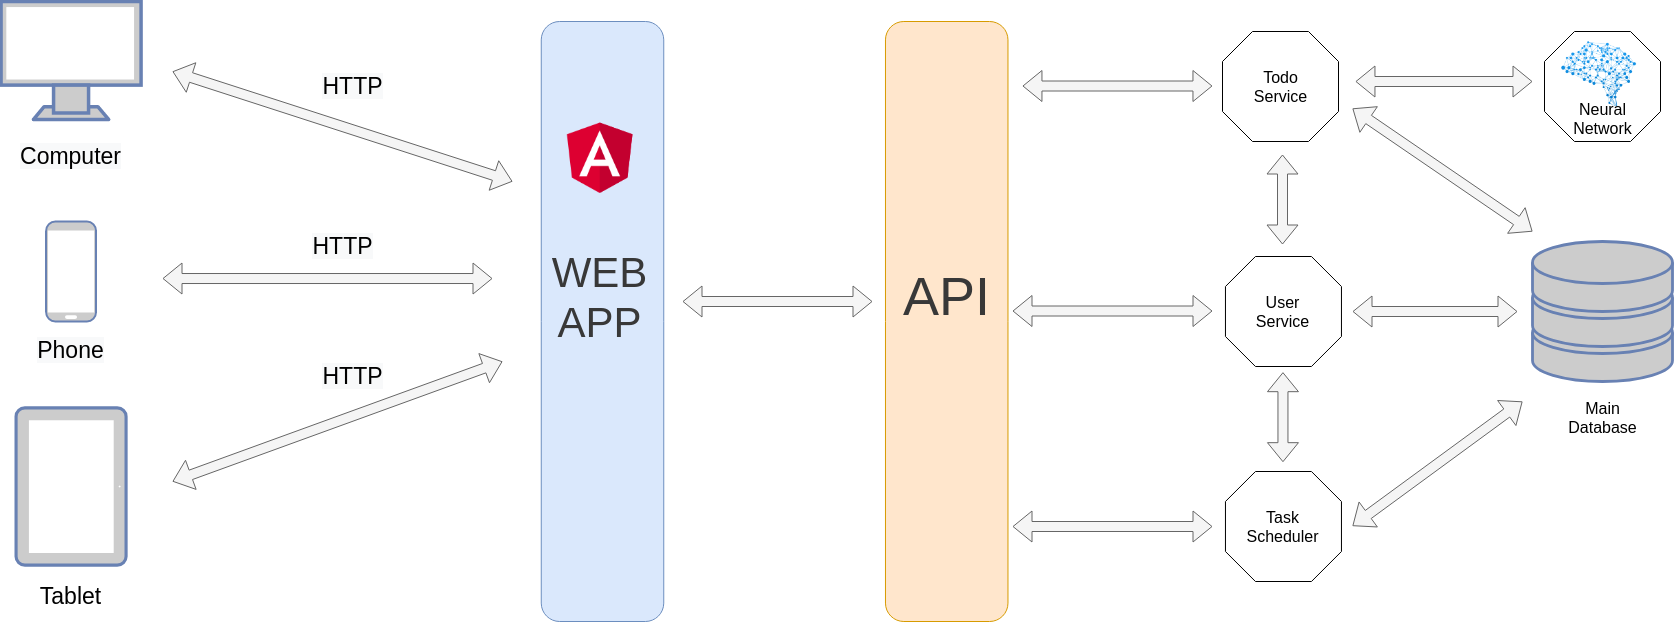
\includegraphics[width=80mm,scale=0.5]{images/abstract_architecture.png}
			\caption{Abstract architecture of the solution}
		\end{figure}
		\vspace{0.5cm}
		The proposed solution is intended to be generic and expandable for future use.
		The user will be able to create, delete and edit new reminders or "to-do's" and assign them a priority as well as a date. The application will then rank these to-do's and arrange them in a way where the user will not forget them and will actually fulfill them.
		
		This will be achieved using a \textit{\cite{REST}} \textit{API} with a push notifications component. There will be a ranking algorithm designed to prioritize these "to-do's" and then remind the user to fullfil them.
		The 
		% The web \textit{API} will be a \textit{REST} \textit{API} composed of 4 layers. The controllers (endpoints), the business layer, the third-party \textit{API} consumers (ie the solvers) and the data access layer (\textit{DAL}) as is shown in the image below. This will be done using the \textit{.NET \cite{dot_net}} and \textit{MVC \cite{mvc}} frameworks. The \textit{DAL} will be using the framework Hibernate \cite{hibernate} as a way to simplify and improve future development. 
		% The database will be constructed using \textit{SQL} Server\cite{sql_server}.
		
		
	\section{Required Functionalities}
		\begin{enumerate}
			\item Allow users to sign up, log in, log out and delete the account.
			\item Create, edit and erase to-do's. 
			\item Push notifications.
			\item Rank to-do's based on date and priority.
			\item Image recognition creation based on physical to-do's (English only).
		\end{enumerate}
	
	\section{Optional Functionalities}
		\begin{enumerate}
			\item Different to-do lists based on categories.
			\item OpenCv
			\item \textit{OpenId \cite{openid}} log in.
			\item Profile Picture.
		\end{enumerate}
	\bigskip
	\section{Schedule}
	\pagebreak
	\bibliographystyle{plain}
	\bibliography{pp}


\end{document}